\begin{quote}
The wide perspective opening up, if we think of applying this science
to the statistics of living beings, human society, sociology and so
on, instead of only to mechanical bodies, can here only be hinted at
in a few words. \cite{Boltzmann}
\end{quote}


Describing the behavior of a large system composed of a large number of small parts for which we know the rules of individual behavior is the main theme of statistical mechanics. It is successful in this regard because at large system sizes the variation in individual behavior, for which we despite knowing the rules we can not measure precisely, is irrelevant: the aggregate quantities are robust and predictable. However, there is no reason to believe this applications are limited to the traditional physics jurisdiction of gases, condensed matter, etc. Any system large enough that its uncertainties can be aggregated into robust properties can be studied using the tools of statistical mechanics: proteins composed of hundreds of aminoacids have a very large number of ways to fold themselves in three dimension, but the rules of attraction for individual aminoacids makes it possible to calculate the probability of certain folding configurations \cite{bryngelson1987}; The opinion of an individual is impossible to predict and model precisely, but the voting patterns or the opinion on moral issues of a nation comprised of millions of unpredictable individuals can be modelled with good accuracy \cite{galam2008, Jerico14}; An aggregation of neurons with local firing rules can generate a neural network capable of storing and remembering patterns \cite{hopfield1982}.

This large range of applications was made more explicit when E.T. Jaynes showed that the methods of statistical physics can be derived not only as a consequence of thermodynamics and physical laws but as the solution of an inference problem following Shannon's Information Theory \cite{Jaynes57}. A century later Boltzmann's prescience turned out to be accurate.

In Economics, traditional theory usually describes the behavior of economic actors such as consumers and firms as the result of rigorous mathematical deduction from a few starting axioms of behavior. From there, one typically deduces the properties of an economy by treating this behavior as the average representative of a larger set of actors. However, this is only valid when interactions among actors is very negligible. When economic actors interact, as they often do, the possibilities are much richer than the representative agent approach allows \cite{Bouchaud13}. A Statistical Mechanics approach could greatly contribute to the field of Economics since it allows for the study of very complex systems, exhibiting rich behavior such as phase transitions, criticality and glassy phases, which are not found in the usual economic models.

The aim of this thesis is to make the case that the intersection of these two fields has a very large potential, being essentially two domains of knowledge that study very similar problems with different dressings: the properties and characteristics of interacting systems. 

\section{Results of this thesis}

The second part of the thesis concerns the three problems worked during this PhD: \emph{(i)} an approach for consumers that do not strictly maximize their utility in the Random Linear Economy model, \emph{(ii)} comparison of the Input-Output tables for real world countries and the ones obtained in the random economies and \emph{(iii)} the impact of inequality when randomly trading goods of different prices. We now briefly describe each of them.

\subsection{Inefficient consumer in a general equilibrium setting}

In Chapter \ref{cha:inefficient} we extend the Random Linear Economy model introduced in Chapter \ref{cha:RLE} by considering the cases where the consumer does not strictly maximizes his utility when choosing a bundle of $M$ goods $x = (x_1, \ldots, x_M)$, starting from his endowment $x_0 = (x_1^0, \ldots, x_M^0)$, in a market composed of $N$ firms each with a random technology $\xi_i = (\xi_i^1, \ldots, \xi_i^M)$ and scalar scale of production $s_i \geq 0$. In the original model, the consumer's choice $x$ is given by the Gibbs distribution at the zero temperature limit, that is,

\begin{equation}
    x^\ast = \argmax_x \lim_{\beta \to \infty} \frac{1}{Z} e^{\beta U(x)} \delta (x - x_0 - \sum_{i=1}^N s_i \xi_i)
\end{equation}

\begin{figure}[!ht]
  \centering
  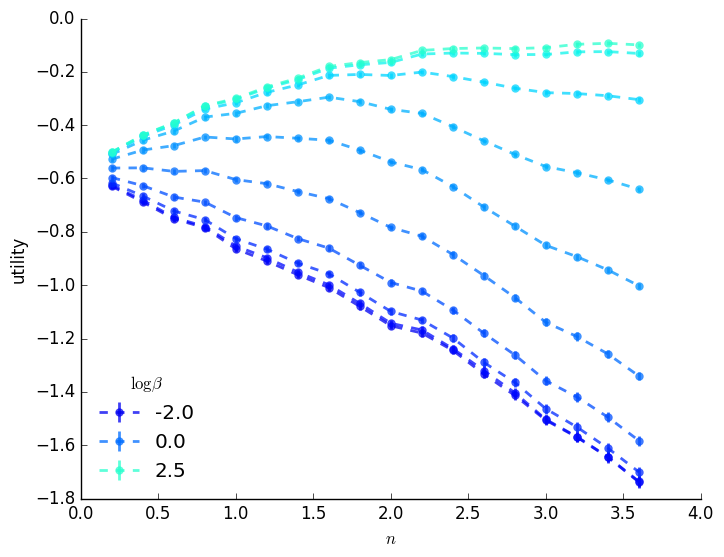
\includegraphics[width=0.45\textwidth]{figs_inef/utility.png}
  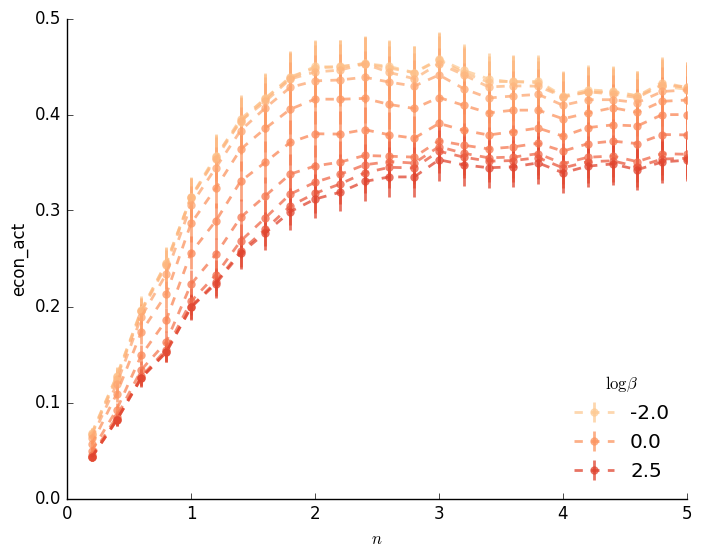
\includegraphics[width=0.45\textwidth]{figs_inef/econ_act.png}
  \caption{\textbf{(Left)} Average consumer utility per good as a function of the number of technologies per good $n$, for several degrees of inefficiency $\beta$ (when $\beta \to \infty$, the consumer strictly maximizes his utility). A large $n$ means there are more trades available for the consumer and a rational consumer should always increase his utility when faced with a growing number of possibilities. This is not the case for a consumer that chooses inefficiently. \textbf{(Right)} Average economic activity (volume of goods exchanged per good) as a function of $n$, for several degrees of inefficiency. An inefficient agent may choose poorly when faced with many choices, but he trades a larger quantity of goods.}
  \label{fig:intro_inef}
\end{figure}

We make the case that the best way to model a suboptimal utility choice is by removing the zero temperature limit, or $\beta \to \infty$, and adjust how much the consumer deviates from "rational" behavior by changing $\beta$. By lifting this simple restriction we  obtain nontrivial behavior, as shown on Figure \ref{fig:intro_inef}. On the left, we show the agents utility as a function of the number of technologies per good $n = N/ M$ for different values of $\log \beta$. When $\beta$ is large (around $10^2$), the agent optimizes efficiently enough that his utility always increases with $n$. However, when $\beta$ gets lower and the representative consumer starts making worse choices (according to his utility function), his expected utility in the market \textit{decreases} with $n$ instead of increasing.

This result corroborates an increasing number of empirical results from Behavioral Economics where the amount of choice a consumer faces may decrease the quality of his choices \cite{Lepper00, Schwartz02}. What is more interesting is that the economic activity in the market, in this case measured by the density of goods being exchanged, \textit{increases} with the inefficiency in consumer choice, because he deviates a lot more from $x_0$ than if he were strictly maximizing his utility. In this stylized economy, markets with agents that make bad decisions have unhappier agents but are more active and, considering economy activity is usually correlated with wealth, richer.

This work has been submitted as Jericó, J.P., Vicente, R. (2016) \emph{Information inefficiency in a random linear economy model}. Europhysics Letters



\subsection{Input-Output of random economies and real world data}

In Chapter \ref{cha:IO} we collect several years of the Input-Output tables for ten real world economies, which are matrices showing how much the industries of each sector of the economy produce and use as input of every good in the economy. The goods are also divided in the same sectors as the industries, in the case of the US at three levels of aggregation: detailed level, with 389 sectors, aggregated with 71 and summary with 15, going from "Mining" in the summary level to "Coal mining", "Iron, gold, silver mining", etc, in the detailed level, and at two levels of aggregation for the EU countries: 64 and 10 levels.

From these Input-Ouput tables we are able to build the Direct Requirement matrices, in which each element represents many dollars of a good are needed to produce a dollar of another good. These matrices represent directed, weighted graphs with the goods as nodes, and by definition the indegrees (sum of all edges that point to the node) are equal to one. The outdegrees, however, are variable, and they indicate the dependency of the production network on a specific good. Acemoglu et al \cite{Acemoglu12} show that the heavier tailed the outdegree distribution is, the more susceptible to shocks is an economy.

\begin{figure}[!ht]
  \centering
  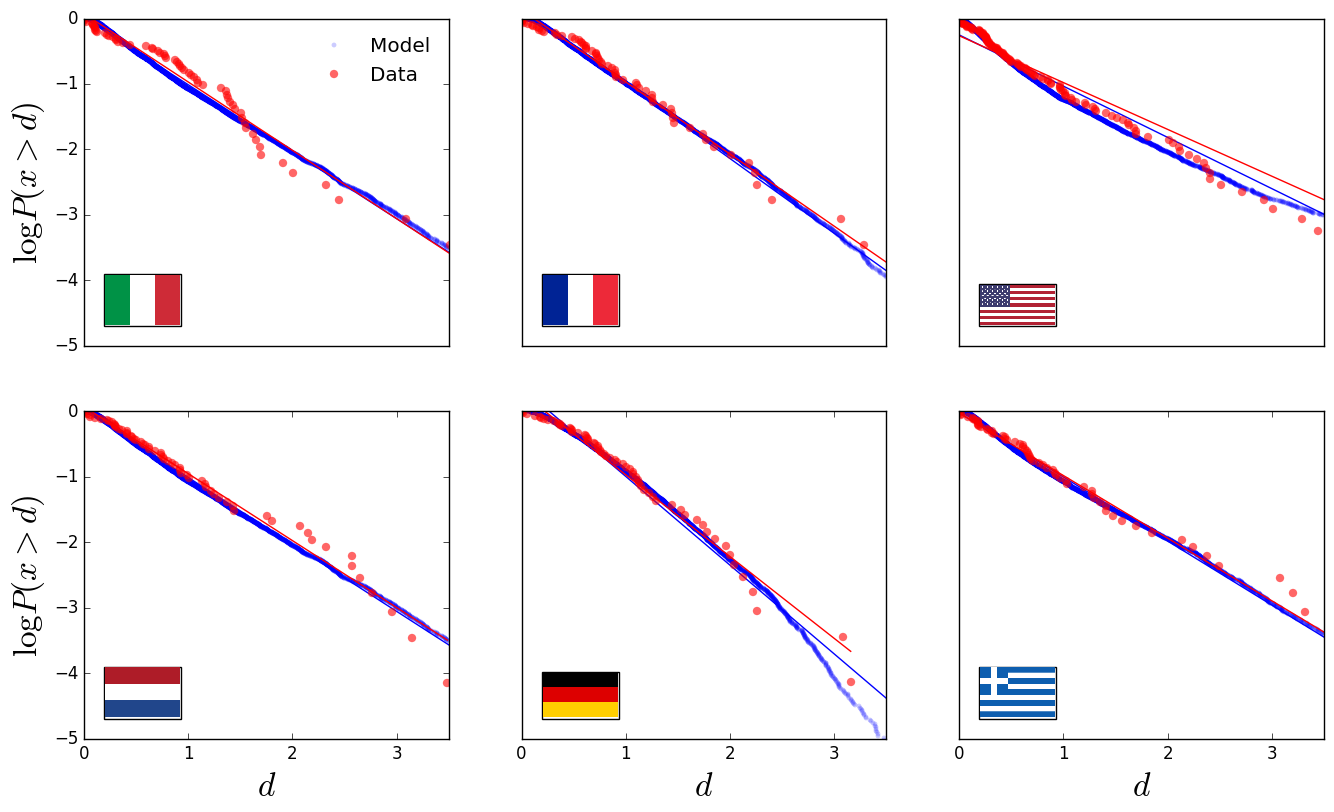
\includegraphics[width=0.95\textwidth]{figs_io/6panel_intro.png}
  \caption{Log of the counter cumulative degree distribution for six of the ten countries analyzed, compared with the closest degree distribution generated by the Random Linear Economy model with $M=100$, $\beta \to \infty$ for different values of $n$. Both datasets are plotted along with their regression, which is very close to an exponential distribution.}
  \label{fig:intro_io}
\end{figure}

We show that the outdegree (or simply degree) distribution of ten countries we have analysed at the aggregated level (64 sectors for the EU, 71 for the US) is very close to an exponential distribution, whereas data at the detailed level of aggregation for the US has much heavier tails. Given that these degrees are random variables with a fixed average, Information Theory tells us that in the absence of any extra constraints the distribution that maximizes entropy is an exponential distribution. This allows us to conjecture that the aggregation process has washed out the structural information of the economy.

We check this hypothesis by generating the Input-Output matrices, and consequently the Direct Requirement matrices, for artificial economies generated by the model introduced in Chapter \ref{cha:RLE} and showing that their aggregation produces the same patterns we observe in real world data. Furthermore, we show that different methods of aggregation yield different results, and the one employed in real world data is closer to random than to one that takes input and output correlations into account. This has a direct consequence on Acemoglu et al's conclusion for the structural fragility of the US economy: distribution tails that were taken into account may have been a simple artifact of the aggregation process, and the real distribution may be heavier tailed than what they calculated. If this is the case, the predictions made on \cite{Acemoglu12} concerning the fragility of the U.S. economy to random shocks may have been underestimated.

This work was accepted for publication as Jericó, J.P., Marsili, M. (2016) \emph{Input Output of random economies and real world data}. Eur. Phys. J. Special Topics: Can economics be a physical science?


\subsection{When does inequality freeze an economy?}

In Chapter \ref{cha:inequality} we show the statistical effects of inequality in a simple trading economy where we have $N$ agents with a initial capital that is power law distributed $P(c_i > c) \sim c^{-\beta}$, and agents trade $M$ goods each with its own price $\pi_1, \ldots, \pi_M$, such that the leftover cash of an agent is its capital $c_i$ minus the price of the goods he owns. At each trading step, one of the $M$ goods is chosen at random and its owner tries to sell it to another agent, which automatically accepts it if he has enough cash to do so.

The parameters are set in such a way that even the most expensive good is affordable to the poorest agent. Despite that, in the stationary state we show that this zero intelligence dynamic divides the agents into "classes" where an agent can afford goods up to a certain price and none more expensive than this threshold. If we define an agent's leftover cash as his liquidity in the market, given a unequal distribution of capital the economy's liquidity concentrates into fewer agents, and as the inequality parameter $\beta$ goes to one, the economy freezes completely as only the richest agents carry any meaningful trade.

\begin{figure}[!ht]
  \centering
  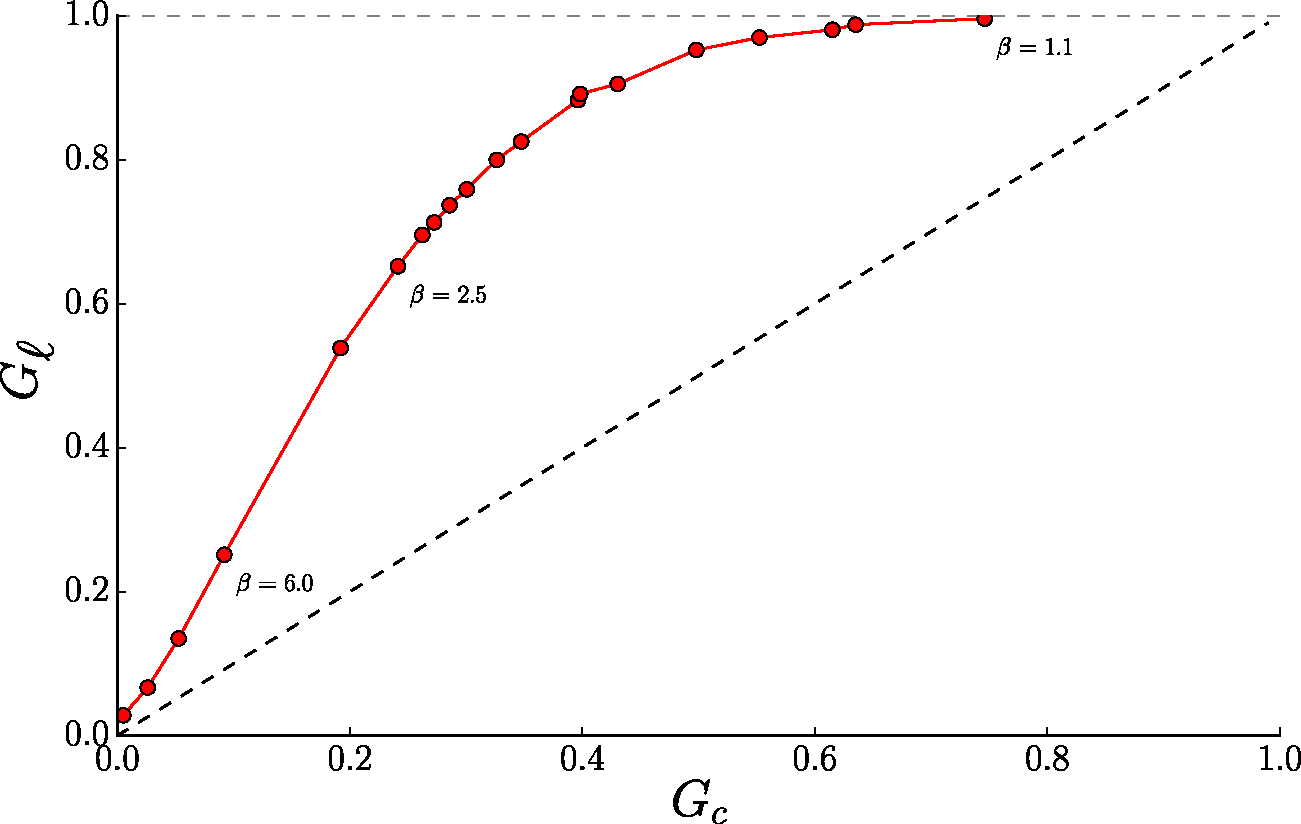
\includegraphics[width=0.65\textwidth]{figs_ineq/gini_intro.pdf}
  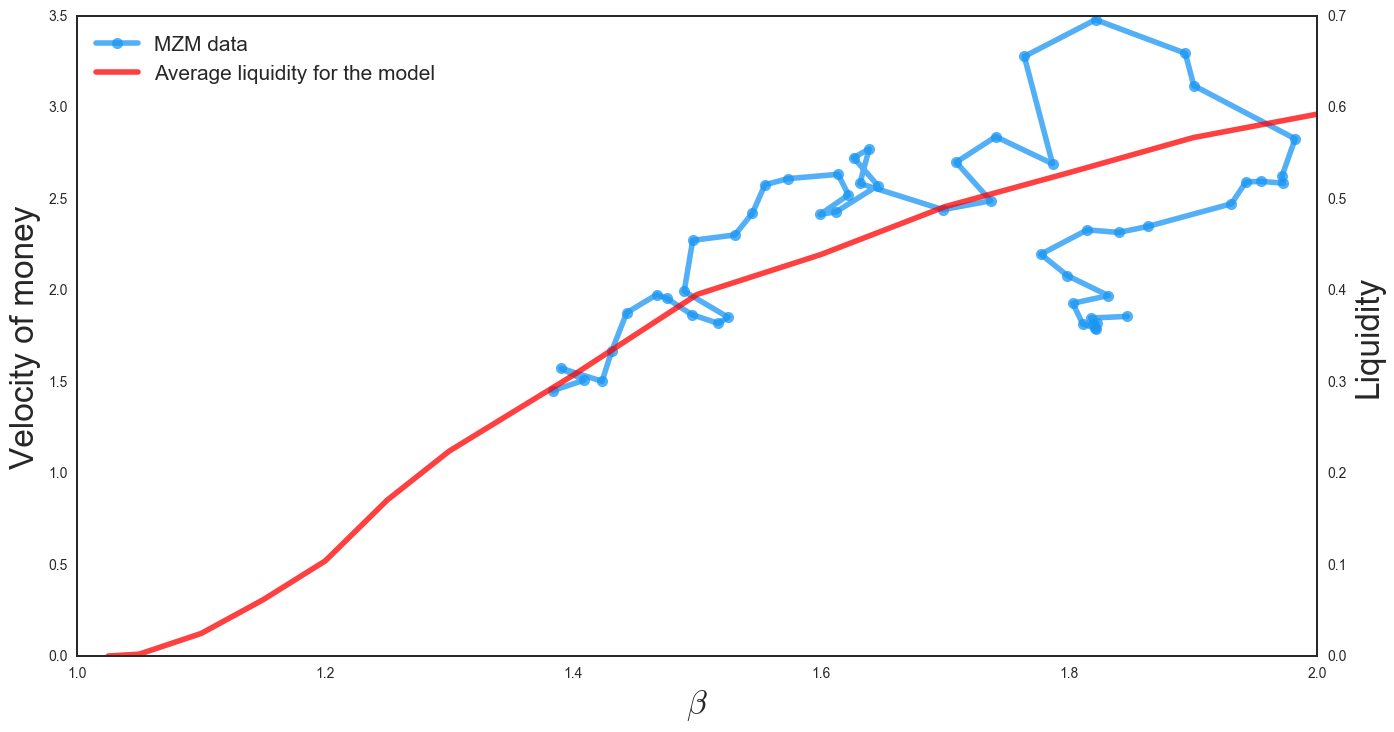
\includegraphics[width=0.65\textwidth]{figs_ineq/data_model.png}
  \caption{\textbf{(Top)} Gini coefficient $G_\ell$ of the cash distribution (liquid capital) in the stationary state as a function of the Gini $G_c$ of the capital distribution, for numerical simulations described in Chapter \ref{cha:inequality}. Cash, or liquidity, is always more unequally distributed than capital, resulting in perfect inequality (when only a countable number of agents have non zero liquidity) when $\beta$ approaches one. \textbf{(Bottom)} Velocity of money, defined for the model by equation \eqref{def:pavg}, as a function of the level of inequality represented by the power law parameter $\beta$, with comparison to the historical US data. Our model corroborates the fact that as inequality increases, the number of money units that are exchanged in a time interval decreases.}
  \label{fig:intro_ineq}
\end{figure}

These results are summed up by the top panel of Figure \ref{fig:intro_ineq}. There we plot the Gini coefficient for the cash as a function of the Gini coefficient for the capital. The Gini coefficient is a measure of inequality in a distribution and goes from zero to one: zero means perfect equality, all data in the dataset are the same. One means perfect inequality: only one point is positive and the rest is all zero. In Figure \ref{fig:intro_ineq}, we show that liquidity in the model is always much more concentrated than the initial capital, converging to perfect inequality when $\beta \to 1$. This has an arresting effect where all trade in the economy stops. This result is tested versus empirical data in the bottom panel of Figure \ref{fig:intro_ineq}, where we compare the velocity of money, as defined by the US Federal Reserver Bank, as a function of the inequality for the model and the historical US data, showing that there is good corroboration that inequality indeed decreases the velocity of money.


This work was published at Jericó, J.P., Landes, F. P., Marsili, M., Castillo, I.P. and Volpati, V. (2016) \emph{When does inequality freeze an economy?}. Journal of Statistical Mechanics: Theory and Experiment, Volume 2016.



\section{Organization of this thesis}

The first part of the thesis will concern the theoretical context of this work, along with some examples in the literature: in Chapter \ref{cha:GET} we will go over a brief introduction of General Equilibrium theory and mainstream Economics research in general. The main aim of the chapter is to give readers of a Physics background the necessary context to understand the standard protocol in Economics when studying a problem, what are some important questions in the field, what techniques are usually used, etc. Our goal is that after reading the chapter, the reader will be convinced of the proximity between the two fields, and how the methods differ despite their aims being essentially the same. 

In Chapter \ref{cha:stat_mech}, we will make the case of why Statistical Mechanics is a suitable tool for exploring and studying Economics. Although the Physics minded reader most likely does not need much convincing, it is still useful for those that never had any exposition to a general, information theoretical approach to Statistical Mechanics as introduced by Jaynes \cite{Jaynes57}. We hope that a reader with a background in Economics (and who hopefully did not stop reading the thesis after Chapter \ref{cha:GET}) will agree with us that the methods presented therein offer an alternative to the usual methods in Economics. In this chapter we will also present a number of previous work that have already explored this intersection.

We end the first part by introducing the Random Linear Economy model in Chapter \ref{cha:RLE}, which consists of a simple market model where companies have random technologies and one consumer wishes to improve his utility by trading his current goods in the market, which is exactly the sort of problem General Equilibrium Theory describes. Despite its simplicity, the model exhibits a rich behavior due to the stochasticity introduced in the technologies and its solution is arrived at by using techniques from the Physics of disordered systems. Its introduction merits a dedicated chapter because not only it serves as the basis for the work developed on Chapter \ref{cha:inefficient} and parts of Chapter \ref{cha:IO}, but also because it is a good representative of the ideas put forward in Chapters \ref{cha:GET} and \ref{cha:stat_mech}.

The second part of this thesis, Chapters \ref{cha:inefficient}, \ref{cha:IO} and \ref{cha:inequality}, are the three problems we have mentioned in the last section. 